%%%%%%%%%%%%%%%%%%%%% chapter.tex %%%%%%%%%%%%%%%%%%%%%%%%%%%%%%%%%
%
% sample chapter
%
% Use this file as a template for your own input.
%
%%%%%%%%%%%%%%%%%%%%%%%% Springer-Verlag %%%%%%%%%%%%%%%%%%%%%%%%%%
%\motto{Use the template \emph{chapter.tex} to style the various elements of your chapter content.}
\chapter{反欺诈:声纹与人脸识别的抗攻击}
\label{basic} % Always give a unique label
% use \chaptermark{}
% to alter or adjust the chapter heading in the running head


这是里关于主题模型和语言模型的介绍。

\section{声纹识别中的抗攻击}

随着声纹识别的应用越来越广泛,声纹识别的安全性要求也越来越高。因此声纹识别研究中,必须了解声纹识别的攻击技术,才能进一步进行防范。在声纹识别应用中,主要的攻击方法分为四大类:模拟(Impersonation)、录播(Replay)、语音合成(Speech Synthesis)和语音转换(Voice Conversion)。

模拟攻击通常来自两种情况:双胞胎和专业模仿人员。双胞胎主要是因为生物信息相对比较接近,所以存在声纹接近的可能。曾经有报道说有双胞胎弟弟用自己声音破解了哥哥在银行的声纹密码。有论文~\cite{patil2005speaker}提到这个问题,从他们的实验结果来看,就算是双胞胎还是存在一定的差异性,能进行区分。对应专业模仿人员,也有数据~\cite{patil2008lp}显示具有声纹攻击性,但是差异比双胞胎大。这一类攻击最大的问题就是可供训练和测试的数据很有限,小数据上能进行防范,但是对于其真正的攻击情况目前认为是不确定的。

录播攻击,一般是用录音机对特定人进行录音,然后播放出来从而达到声纹认证通过的效果。在ASVspoof2017~\cite{kinnunen2017asvspoof}比赛中,通过参赛人的比赛结果以及对往届的比赛结果来看,录播攻击识别难度比语音合成、语音转换攻击识别难度更高。录播攻击其中涉及到录音环境、播放环境、录音设备等干扰,会一定程度对识别是否是攻击造成一定难度。

语音合成攻击,一般分为两类,一个是拼接方式,一个是TTS语音生成方式。针对TTS,机器识别准确一般比较高,因此不会造成比较大的威胁。但是语音拼接,这种技术方式,针对我们人耳能准确识别,但是对于机器而已,他们比较大可能认为是真实说话声音。

语音转换是把一个人说话的录音改变音色,频率等转换为具有另外一个人说话特点的技术~\cite{jia2018transfer}。一般会用语音转换和TTS技术进行结合进行攻击,这样能比较方便有效,相对攻击成本比较低。这种攻击方式通常都能识别出来,机器生成的毕竟存在一定模式规律。但是也会存在一种风险,这种防止攻击的鲁棒性不一定很高。

针对这一系列的攻击方法,通用的抗攻击框架是在声纹识别前增加一个前置模块,用来专门识别是否是攻击。目前业界对这些攻击方式能较为准确识别,但是需要不断积累足够大的样本,从而提高更高的防护能力。


\section{人脸识别中的抗攻击}

人脸活体检测( Face Anti-Spoofing)技术是人脸识别系统中,用以确认待认证对象是否为真实生物活体的一项技术。一方面,人脸识别技术的商业化愈加成熟和广泛,极大改善和推进了社会金融活动的智能化和便捷性;另一方面,由于人脸照片、视频数据相对容易获取和复制,若无活体检测这一环节,那么使用被盗取的合法用户的照片、视频或者3D面及头套等即可入侵人脸识别系统,由此将带来极大危害\cite{chingovska2012effectiveness}。在目前的人脸识别系统中,常见的活体检测技术包括动作活体、3D活体、红外活体、光线活体等。下面将逐一简单介绍。

动作活体是通过利用人脸关键点和人脸跟踪等技术,检测用户眨眼、张嘴、摇头等多种动作及其组合,可有效抵御照片、换脸、面具、遮挡以及屏幕翻拍等常见的攻击手段,但较难抵御视频回放攻击。

3D活体通过专用硬件(例如3D结构光、ToF等)获取人脸部3D结构信息,可以有效防御如手机、电脑等屏幕显示和打印照片等2D攻击手段,但是需要配合其他方法抵御近几年出现的高质量3D面具攻击\cite{zhang2019dataset}。

红外活体检测一般利用人体皮肤对近红外光的反射率较高,相比于其他材质有明显区别的特性,通过专用红外设备获取人脸部红外图像判断是否为活体。实际应用中通常使用主动红外摄像,即通过红外LED照射人脸,利用红外摄像头获取人脸部图像,分类判断是否为活体。红外活体检测技术对于常见攻击手段具有较好的防御效果,缺点在于需要特定红外设备\cite{zhang2019dataset,yi2014face}。

光线活体是近两年出现的一种活体检测技术。由于3D活体、红外活体需要特殊设备,在已有系统中部署较为困难。光线活体技术利用屏幕发出不同颜色和强度的光线照射在人脸上,由于人脸自身的三维结构以及皮肤等生理组织对于不同颜色光线的反射率不同,从获取的视频中提取相应的活体信息,如图\ref{fig:light_reflection}所示。这项技术由于无需特殊硬件设备、且具有较高的准确率,在手机等移动端使用较为方便。其缺点在于要求视频拍摄过程稳定,闪光带来的用户体验需要得到提升,同时户外强光也会带来较大干扰\cite{liu2019aurora}。

\begin{figure}[ht]
\centering
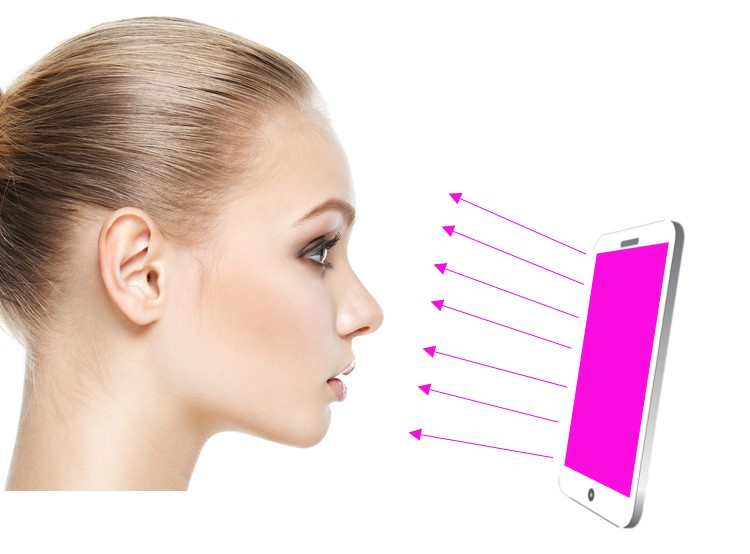
\includegraphics[scale=0.5]{img/chapter_as/light_reflection.jpg}
\caption{光线活体}
\label{fig:light_reflection}
\end{figure}
